\paragraph{QuizziPedia::Front-End::Controllers::QuizEventController}
\begin{figure} [ht]
	\centering
	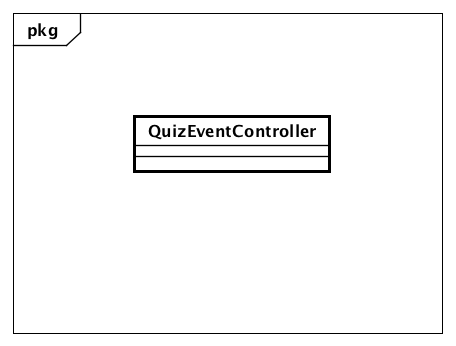
\includegraphics[scale=0.45]{UML/Classi/Front-End/QuizziPedia_Front-end_Controller_QuizEventController.png}
	\caption{QuizziPedia::Front-End::Controllers::QuizEventController}
\end{figure} \FloatBarrier
\begin{itemize}
	\item \textbf{Descrizione}: questa classe permette di reagire ai comandi dell'utente durante la gestione dei suoi questionari;
	\item \textbf{Utilizzo}: fornisce le funzionalità per reagire ai comandi dell'utente, effettua redirect alle pagine richieste, come la visualizzazione delle statistiche di un questionario e iniziare un questionario in modalità esame.
	\item \textbf{Relazione con altre classi}:
	\begin{itemize}
		\item \textit{IN} \texttt{EliminationAndModifyDirective}: componente grafico contenente i bottoni per eliminare o modificare un questionario;  
		\item \textit{IN} \texttt{ExamModalityDirective}: directive contenete i componenti grafici per attivare la modalità esame su un questionario e gestire le iscrizioni;
		\item \textit{IN} \texttt{QuestionnaireResultsDirective}: rappresenta il componente grafico che permette all'utente autenticato pro di vedere i risultati di chi ha compilato il questionario. Tale componente è contenuto nella lista dei questionari abilitati alla compilazione. \'E possibile accedere alla lista dei risultati azionando l'evento ad esso collegato;
	\end{itemize}
	\item \textbf{Attributi}:
	\begin{itemize}
		\item \texttt{-} \texttt{\$scope: \$scope} \\
		Campo dati contenente un riferimento all’oggetto \$scope creato da \textit{Angular\ped{G}}, viene utilizzato come mezzo di comunicazione tra il controller e la view. Contiene gli oggetti che definiscono il model dell’applicazione;
		\item \texttt{-} \texttt{\$location: \$location} \\
		Campo dati contenente un riferimento al servizio creato da \textit{Angular\ped{G}} che permette di accedere alla barra degli indirizzi del \textit{browser\ped{G}}, i cambiamenti all’URL nella barra degli indirizzi si riflettono in questo oggetto e viceversa;
		\item \texttt{-} \texttt{\$mdDialog: \$mdDialog} \\
		Campo dati contenente un riferimento al servizio della libreria \textit{Material for Angular\ped{G}} che permette di creare delle componenti a popup;
	\end{itemize}
	\item \textbf{Metodi}:
	\begin{itemize}
		\item \texttt{+} \texttt{QuizEventController(\$scope: \$scope, \$location: \$location, \$mdDialog: \$mdDialog)} \\ Metodo costruttore della classe. \\
		\textbf{Parametri}:
		\begin{itemize}
			\item \texttt{-} \texttt{\$scope: \$scope} \\
			Parametro contenente un riferimento all’oggetto \$scope creato da \textit{Angular\ped{G}}, viene utilizzato come mezzo di comunicazione tra il controller e la view. Contiene gli oggetti che definiscono il model dell’applicazione;
			\item \texttt{-} \texttt{\$location: \$location} \\
		    Parametro contenente un riferimento al servizio creato da \textit{Angular\ped{G}} che permette di accedere alla barra degli indirizzi del \textit{browser\ped{G}}, i cambiamenti all’URL nella barra degli indirizzi si riflettono in questo oggetto e viceversa;
			\item \texttt{-} \texttt{\$mdDialog: \$mdDialog} \\
			Parametro contenente un riferimento al servizio della libreria \textit{Material for Angular\ped{G}} che permette di creare delle componenti a popup;
		\end{itemize}
		\item \texttt{+} \texttt{modifyQuestionnaire(quizId: String): void} \\
		Metodo che gestisce l’evento click sul pulsante di modifica questionario. Effettua il redirect alla pagina di gestione questionari;
		\begin{itemize}
			\item \texttt{quizId: String}: parametro che indica l'identificativo univoco di un questionario.
		\end{itemize}
		\item \texttt{+} \texttt{deleteQuestionnaire(quizId: String): void} \\
		Metodo che gestisce l’evento click sul pulsante di eliminazione questionario. Effettua il redirect alla pagina di gestione questionari;  
		\begin{itemize}
			\item \texttt{quizId: String}: parametro che indica l'identificativo univoco di un questionario.
		\end{itemize}
		\item \texttt{+} \texttt{subscribeManagement(quizId: String): void} \\
		Metodo che gestisce l’evento click sul pulsante di gestione iscrizioni. Effettua il redirect alla pagina di gestione iscrizioni; \\
		\textbf{Parametri}:
		\begin{itemize}
			\item \texttt{quizId: String}: parametro che indica l'identificativo univoco di un questionario.
		\end{itemize}
		\item \texttt{+} \texttt{examModalityquizId: String(): void} \\Metodo che gestisce l’evento click sul pulsante di attivazione modalità esame. Effettua il redirect alla pagina di gestione questionari; \\
		\textbf{Parametri}:
		\begin{itemize}
			\item \texttt{quizId: String}: parametro che indica l'identificativo univoco di un questionario.
		\end{itemize}
		\item \texttt{+} \texttt{resultsQuestionnaire(quizId: String): void} \\
		Metodo che gestisce l’evento click sul pulsante di allenamento. Effettua il redirect alla pagina di gestine questionari;
		\begin{itemize}
			\item \texttt{quizId: String}: parametro che indica l'identificativo univoco di un questionario.
		\end{itemize}   
	\end{itemize}
\end{itemize}